\chapter{Review of Related Literature}
\label{sec:relatedlit}

This chapter will present the different methods and approaches of related LEGO instruction manual systems. The decision of AR usage will also be discussed.

\section{Augmented Reality over Paper-based Manuals}
The paper-based and digital-based manual both shows a layer-by-layer brick representation. The digital-based manual gives the user the ability to rotate, scale, and translate the assembly manual. On the contrary, paper-based manuals are rendered with a fixed view position by parallel projection therefore it is easier to understand or be visualized \cite{Tseng:2012:BEM:2307096.2307119}.

Hou et al. conducted a research to see if the use of AR can help an assembler cognitively. Two types of experiments with two sub-types each were conducted. One experiment focused on the type of guidance gets whilst building the LEGO model itself, while the other experiment focused on the type of training a builder has to go through first before building a LEGO model without guidance. Each experiment was used to compare the inclusion and exclusion of AR as a substitute for paper-based manuals. Results from these experiments indicated a positive effect of the cognitive facilitation when using an animated AR system. When AR was used, the learning curve of trainees significantly improved, and fewer errors were made \cite{HouWangBernold2013}.
    
    An AR based manual will instantly display the component it is referring to. Given the visualization of the current state of the object will reduce the search time in assembly. Furthermore, AR would lessen the effort of the user in reading textual information. The amount of attention switching would be minimized and would increase productivity. Lastly, AR could possibly resolve ambiguities through indicators that shows the proper location of a certain component\cite{AR-Context}.

\section{Augmented Reality Technologies}
This section will discuss the various technologies that will be correlated with the use of AR. 
\subsection{Object Recognition/Tracking}
Nishira et al. proposed an augmented reality system that guides users in assembly tasks through image processing techniques to recognize the pieces and guide the piece placement with graphic signs\cite{nishihara_okamoto_2015}. Their proposal planned to first capture the camera image from a tablet then through the OpenCV library\cite{791289}, calibrate and undistort the image. Through image processing, pieces shown in the image are then segmented. Perspective distortion are then rectified as features and computer invariants are extracted. Their system then matches the piece to their model. Their system then shows through AR the assembly to be created, and highlights the place where the matched piece should be placed. This then gets repeated until the final assembly state is achieved. What they were able to create however, was a system that could identify 12 pentomino parts with their corresponding labels through a tablet's camera.

\section{Assembly Instructions through AR}
In general, in manufacturing quality assessment and final inspections are usually done manually despite the advancement of technology requiring less human effort. On the other hand, productions that require manual assembly are usually done by operators that are especially trained to do these kinds of procedures. In the effort to save time and resources on having to conduct trainings, the number of guiding tools that help manual assembly continue to increase given that studies prove it improves the efficiency of manual assembly \cite{Wang2016406}.

Meanwhile, some assembly guide systems are AR-assisted. Each AR-based assembly guiding system proposed and implemented has its own way of managing instructions. These systems augment the user's view to ease the assembly processes and use various types of medium\slash tools such as head mounted display, marker, stylus among many other gears.There are also assembly systems that require the user to use specific hand gestures for its different commands and functions. An example where hand gestures are used is the study of Wang et al. They built a multi-modal assembly guidance that facilitate the assembly processes through EBHI. Sample hand gestures used in the proposed system are found in Figure 2.1.

\begin{figure}[h!]
  \centering
  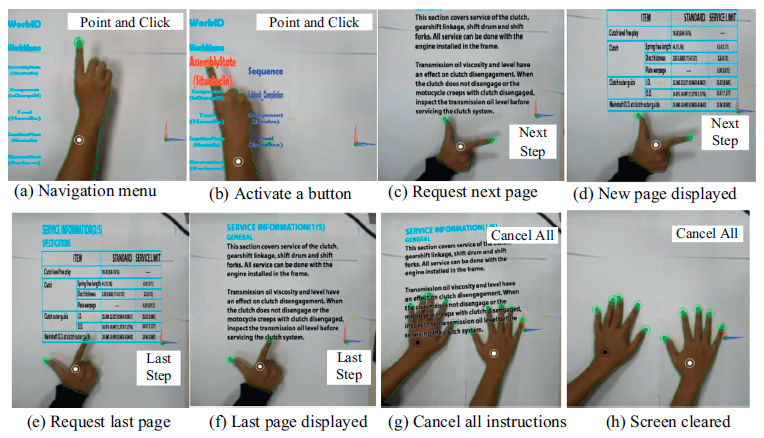
\includegraphics[width=1\textwidth]{SampleHandGestures}
  \caption{Sample hand gestures used in the assembly guidance (Wang et al., 2016).}
\end{figure}

With the numerous AR-based assembly guidance systems that already exist or have been proposed, a group of people published a paper under IEEE regarding guidelines on the creation of instructions that would help this research develop the augmented portion of the generation of the instruction manual. Instructions are denoted by the researchers as a system's way of relaying information and giving feedback to the user. For most of the study's main discussion,ِ AR systems ideally need the following in order to give instructions:

\begin{itemize}
	\item Indicate the correct path, correctness of movement, velocity, or acceleration to indicate the right way to achieve the goal.
    \item Emphasize the blocks or elements to be moved or changed to let the user know which part of the object must be moved.
    \item Allow the customization of visual appearance attributes such that the user could control it, but it is also ideal to leave some tasks that could have specific patterns to follow.
    \item Give feedback; let the user know if the task is done correctly or how much progress has been done with the object.
    \item Manage occlusion and depth especially in cases where the object is three-dimensional.
\end{itemize}

\section{LEGO Assembly Guidance}

Context-aware approaches like the study of Khuong et al. evaluated the effectiveness of an AR-based context-aware assembly support system\cite{6802051}. They stated that context-related visualization of information helps to reduce search time in assembly. They created two AR context-aware visualization modes for the study. One displayed guidance information directly overlaid on the physical model and another featured a virtual model adjacent to the real model. The result was that the visualization mode that rendered guidance information separate from the physical model was preferable over the overlaying visualization mode.












